\chapter{Forecasting the Flow of Human Crowds}

\begin{figure}[tb]
	\centering
	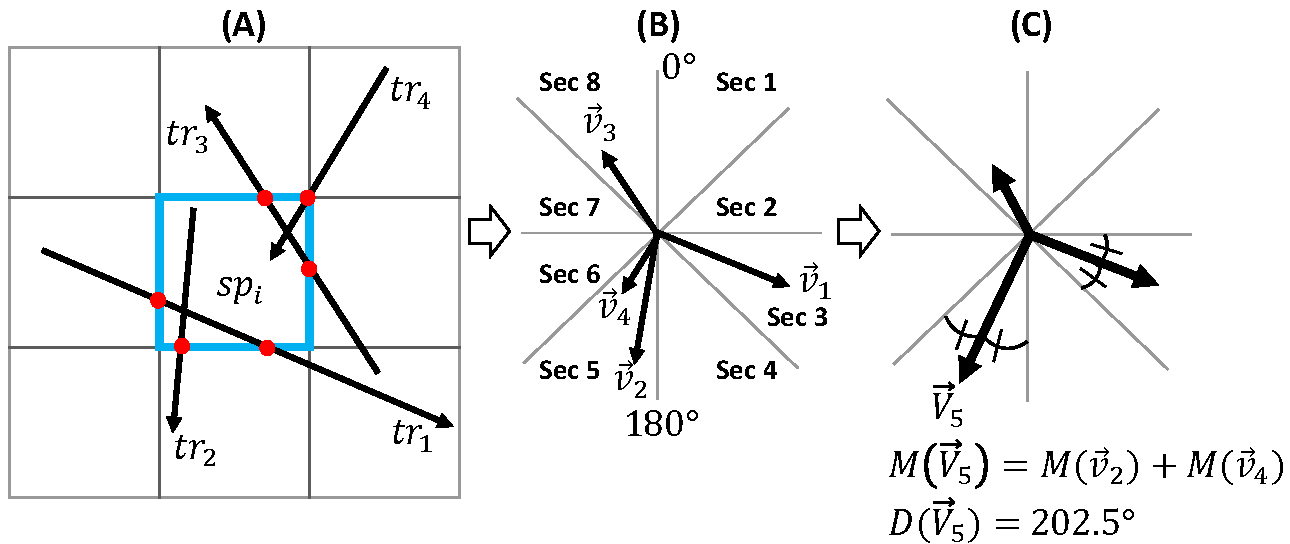
\includegraphics[width=1.0\columnwidth]{discretization}
	\caption{Trajectory tessellation and directional density estimation}
	\label{fig:segment}
	%\vspace{-0.7cm}
\end{figure}

Forecasting human crowd flows plays a significant role in a range of applications, from urban and traffic planning~\cite{Wei:2012:CPR, Zheng:2011:UCW} to predicting epidemic dynamics~\cite{Dalziel:2013:Human, Eubank:2004:Modelling}.
Various location-based services are also highly dependent on foreseeing human movement patterns~\cite{Bao:2012:Location}.
The volume and variety of data that capture the different aspects of human mobility have greatly increased due to ubiquitous crowdsourced activities and the advent of several location-based social networking services.
The potential impacts and availability of such data have caught the attention of researchers from various domains.
They have put considerable efforts into understanding and predicting human mobility patterns~\cite{Gonzalez:2008:UIH,Xue:2013:Destination,Ying:2011:Semantic}.
They have also discovered that human mobility behaviors can contain discernible patterns that can be used for forecasting purposes. 
For example, Song et al.~\cite{Song:2010:Limits} reported a 93\% potential predictability in human mobility from anonymized mobile phone data, and although the overall travel patterns were vastly different, the variability in predictability was found to be significantly low. 

Many previous techniques for predicting human movements have treated the individual mobility behaviors as discrete entities and focused on predicting the next destinations of the individuals based on the observations of their past movement patterns or frequent behaviors of similar users~\cite{Monreale:2009:Wherenext,Xue:2013:Destination,Ying:2011:Semantic}.
While recent work has made progress in predicting human mobility patterns, the proposed models that are based on movements of individuals suffer from many limitations.
%For example, these approaches do not consider the flows (i.e., aggregate movements) as a whole --NOT SURE WHAT THIS MEANS; SUGGEST REMOVE THIS SENTENCE -AM.
For example, the data modeling techniques used in these methods (e.g., Hidden Markov Model) typically require extensive training of the data models using historical observed data~\cite{Mathew:2012:Predicting,Xue:2013:Destination}. 
This process can be expensive and rate limiting, especially in case of large scale datasets (e.g., taxi data in large urban regions), and can further severely restrict interactive visual analytic system behaviors.
%If they need to deal with a large-scale training data set (e.g., taxi trips in a large urban area), the computation cost should highly increase.
Other 
%issues related to utilizing individual trajectory mining techniques for forecasting purposes 
challenges 
include privacy concerns for the individuals~\cite{Monreale:2010:Movement,Xue:2013:Destination}.
Furthermore, the individual spatial sequence trajectory datasets, especially those derived from location-based social networks, can also suffer from data sparsity and noise problems~\cite{Wei:2012:Constructing,Wang:2014:Visual}.
%Particularly the paths extracted from location-based social networks have a high degree of sparsity and noise.
%These limitations can disconnect the continuous flows.
These can often prove to be prohibitive for accurate data modeling.
Standard methods to mitigate for these challenges include clustering techniques that summarize the overall movement paths in trajectory data analysis.
These require analysts to carefully select appropriate abstraction levels for clustering in order to prevent the original vector flow data from getting distorted. 
%if an abstraction level that is too high is used for clustering, the original paths and directions get distorted, resulting in inaccurate results.
%Finally, most of the previous work in data mining and knowledge discovery areas do not concern visualizing and exploring the predicted movements.
However, when these abstraction levels are carefully chosen, the analysis of collective flows of human crowds can provide new insights that may not be available at finer granularity levels~\cite{Andrienko:2013:Visual, Hughes:2003:Flow}.

To this end, this paper presents a space-based approach for forecasting the flow of human crowds.
%We also provide an interactive visual analytics environment which enables effective exploration of the predicted results and further analysis~\cite{Andrienko:2013:Visual,Laube:2014:Computational}.
Our work is motivated by weather simulation and forecasting modeling techniques that are built using local atmospheric observations from weather stations. 
%using the values at locations (usually evenly spaced grid) 
%and then generate an atmospheric simulation for a forecast.
In this work, we embed individual movements into a two-dimensional (2D) Euclidean space and model for the space instead of the moving objects.
In other words, given a space with a large number of moving objects, we discretize the space into smaller sub-spaces and model the movement flows for each sub-space.
Our model forecasts the future flow based on observed historical patterns of each sub-space using a seasonal trend analysis technique~\cite{Cleveland:1990:SAS}. 
We then combine the results to visualize the future flow as a whole for the entire space.
%Our approach does not highly depend on the volume of moving objects.
Our approach consists of a directional flow density estimation method that preserves the original paths and directions of moving entities, and a flow smoothing method based on both local and global trajectory trends to mitigate for the data sparseness and noise issues.
We also provide a novel visualization technique for showing the probability density distribution of flow.
% [IS IT NOVEL? -AM].
We demonstrate our work using location-based social media data and GPS tracking human and taxi data.
% [IS THIS CORRECT?]. 

The main contributions of this work include the following:

\begin{itemize}
	\item We apply a new method to estimate the directional flow density that represents the overall movement direction and preserves the original paths and directions of moving entities.
	\item We develop a new flow smoothing method based on both local and global movement trends for improving forecast accuracy by mitigate the effect of the data sparsity and noise.
	\item We propose a new model to forecast vector field data with the seasonal-trend decomposition technique (STL) by transforming data to a series of magnitude values from the smoothed representative vectors.
	\item We develop a new flow visualization technique of multi-vector fields for the directional flow density in order to expose the uncertainty of the vector field.
\end{itemize}




\begin{figure}[tb]
	\centering
	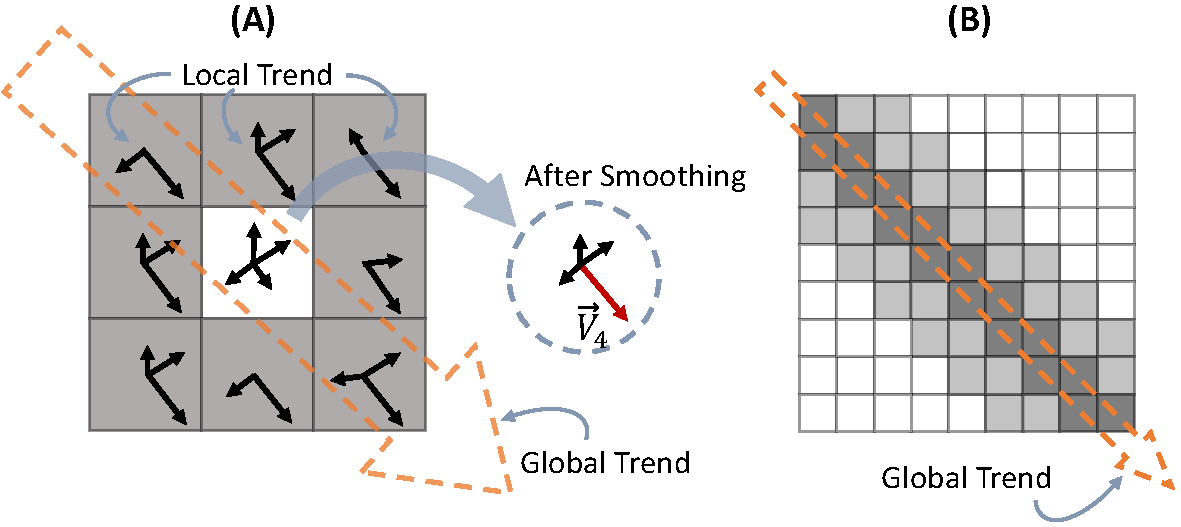
\includegraphics[width=1.0\columnwidth]{smoothing}
	\caption{Each space's directional density is computed based on its neighbors' and global trends. }
	\label{fig:smoothing}
	%\vspace{-0.7cm}
\end{figure}

%
%an interactive visual analytics environment which enables effective exploration of the predicted results.
%
%Our approach enables ...
%Visualization of future flow of human crowds
%Our visualization is able to represent not only major flow, but also minor 


%In this work, our model embeds trajectory data in a two-dimensional (2D) space and then splits the space into discrete grid cells 
%%location entities.
%%We discretize the space through a uniform grid with cells of a specific size.
%%The size depends on the area and the zoom level.
%%For each cell, we transform the sub-part of each trajectory passing through the cell boundary into Euclidean vectors.
%For each cell, we transform the trajectories passing through the cell boundary into Euclidean vectors.
%Then, we summarize the vectors.
%The traditional methods for the summary of vectors, vector addition, vector average, and spherical linear interpolation have a limitation, which results in a small average vector with a meaningless direction when the directions of the vectors with similar magnitude are evenly distributed.
%Our approach is designed as a best-effort method for preserving the original directions of the vectors.
%We divide one full turn (360\degree) into multiple sectors of a same size and then classify each vector into one of the sectors according to its direction.
%Each grid cell will have its directional distribution of the trajectories passing the cell (see Figure~\ref{fig:segment} (B)).
%Then, our model smooths the directional distribution based on local and global trends.
%We adjust the directional distribution of each cell based on the ones of its adjacent neighbor cells and the direction of the global movement around the cell.
%Individual in a crowd tends to follow dominant paths of the crowd~\cite{Kok:2015:Crowd}.
%Our model creates a vector field in the plane consisting of location points with multiple vectors calculated using the directional distributions at each location (see Figure~\ref{fig:segment} (C)).
%Next, We creates a series of vector fields for past time intervals and then predict the future vector fields based on the past vector fields.
%In other words, our model forecasts the future directional distribution of a specific location based on the past ones of the same location using a statistical forecasting technique.
%Then, it repeats the same procedure on each location to create the future vector fields.
%Finally, we visualize the vector fields using particle tracing, a standard flow visualization technique, for representing the future flow of human crowds.


\begin{figure}[tb]
	\centering
	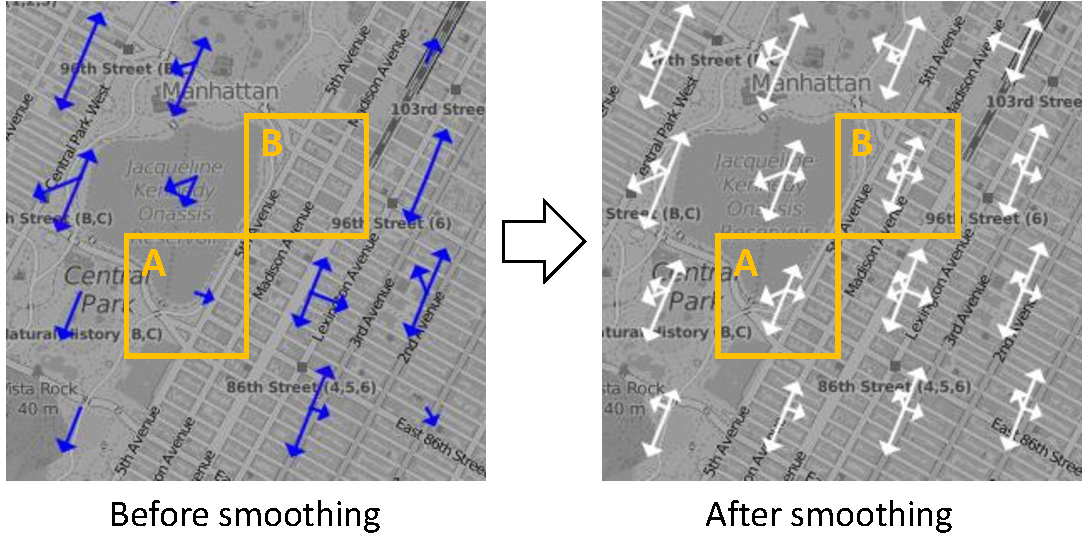
\includegraphics[width=1.0\columnwidth]{smoothdemo}
	\caption{An example of the smoothing result. Sub-space B does not have density due to sparseness data (Left). Sub-space has the density (Right).}
	\label{fig:smoothdemo}
	%\vspace{-0.7cm}
\end{figure}


\begin{figure}[tb]
	\centering
	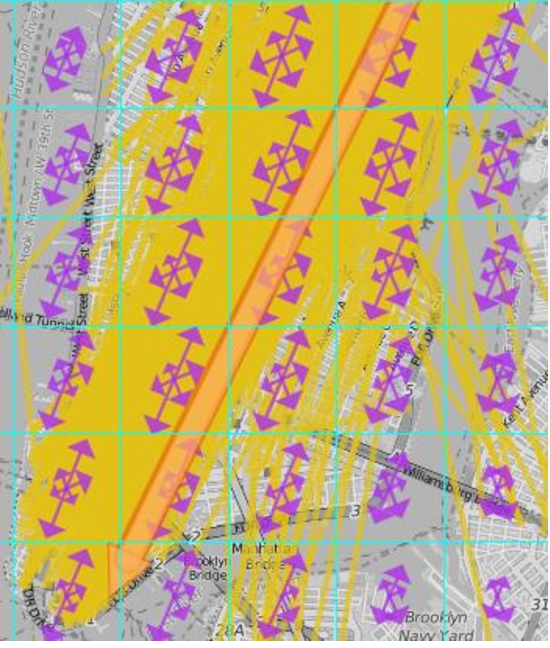
\includegraphics[width=0.6\columnwidth]{nyc_flow}
	\caption{Local directional density (purple arrows) and global (orange arrow) trends of taxi movements in southern Manhattan between 6:00 AM and 10:00 AM.}
	\label{fig:taxi_glyph}
\end{figure}



\section{Flow Data Modeling, Forecasting, and Visualization}

Our flow modeling methodology consists of a pipeline of several processes.
We first apply a directional density estimation technique (Section~\ref{sec:discretization}). 
We then apply a flow smoothing procedure in order to mitigate the data sparseness and noise (Section~\ref{sec:smoothing}).
%At the center of our approach are the methods for computing and smoothing directional density estimation.
After these processes are completed, we forecast the future geospatial flows using the seasonal trend decomposition based on loess technique (Section~\ref{sec:futureflow}) and finally visualize the results using a particle advection technique(Section~\ref{sec:forecasting-visualization}). % and utilize these forecasts the result.
These processes are described in detail in the following sub-sections. 

%AM: I SUGGEST THAT YOU BRING SECTION 4 TO SECTION 3.4.

%We describe these processes in detail below.
%In the next sections, we explain our processing methods and forecasting models to have movement prediction. %First we consider a space over a domain$\Omega\subset \mathbb{R}^{2}$ where a large number of trajectories of a specific time window are projected. Once the data is projected, the given space $\Omega$ are split into multiple sub-spaces $\Omega = \left\{sp_1, \cdots, sp_n\right\}$ in order to estimate and smooth directional density and forecast future flow.
%These methods and models for directional density estimation, smoothing, and forecasting are crucial steps in our computation. We describe those in the next sections in detail. 

%For a given space defined over a domain $\Omega\subset \mathbb{R}^{2}$ in which a large number of trajectories of a specific time window are embedded, we split $\Omega$ into small sub-spaces $\Omega = \left\{sp_1, \cdots, sp_n\right\}$ and estimate the directional density representing the directions of the movements of each sub-space.
%The overall process is illustrated in Figure~\ref{fig:segment}.
%For a given space in which a large number of trajectories are embedded, 
%We discretize the space $\Omega$ through a uniform grid with resolution $R$.
%We discretize the space $SP$ through a uniform grid with cells of a specific size.
%The size depends on the area and the zoom level.
%For each cell, we transform the sub-part of each trajectory passing through the cell boundary into Euclidean vectors.
%For each sub-space $sp_i$, we segment the individual trajectories $tr_i$ passing through the sub-space so each segment is contained on a cell of the grid (see Figure~\ref{fig:segment} (A)).
%Then, we transform the sub-trajectories of $tr_j$ passing through the cell into Euclidean vectors $v_j$ with the same origin point (the center of the cell) (see Figure~\ref{fig:segment} (B)).




%Here is the brief explanation of our forecasting model.
%Our model for forecasting the flow of human crowds consists of the following major steps:
%\begin{enumerate}
%\item embed trajectory data for a time interval into a 2D space, and then, the space is tessellated into square sub-spaces of the same size;
%\item for each sub-space, segment the trajectories so each segment is contained on the sub-space;
%\item transform the trajectory segments into Euclidean vectors and estimate the directional density of the sub-space using the vectors;
%\item smooth the directional density based on local and global directional trends;
%\item create a vector field consisting of location points with representative vectors exhibiting the directional density;
%\item prepare a series of the vector fields for a series of the corresponding past time intervals;
%\item predict the future vector fields for the space based on the series of the past vector fields.
%\end{enumerate}

%The detailed procedure for each step are described in the following sub-sections.

%1) embed trajectory data for a time interval into a 2D space and split the space into discrete grid cells;
%%We discretize the space through a uniform grid with cells of a specific size.
%%The size depends on the area and the zoom level.
%%For each cell, we transform the sub-part of each trajectory passing through the cell boundary into Euclidean vectors.
%2) for each cell, transform the trajectories passing through the cell boundary into Euclidean vectors;
%3) estimate the directional distribution of the vectors in the cell;
%%Then, we summarize the vectors.
%%The traditional methods for the summary of vectors, vector addition, vector average, and spherical linear interpolation have a limitation, which results in a small average vector with a meaningless direction when the directions of the vectors with similar magnitude are evenly distributed.
%%where, our approach is designed as a best-effort method for preserving the original directions of the vectors.
%%We divide one full turn (360\degree) into multiple sectors of a same size and then classify each vector into one of the sectors according to its direction.
%%Each grid cell will have its directional distribution of the trajectories passing the cell (see Figure~\ref{fig:segment} (B)).
%5) smooth the directional distribution based on local and global trends;
%%We adjust the directional distribution of each cell based on the ones of its adjacent neighbor cells and the direction of the global movement around the cell.
%%Individual in a crowd tends to follow dominant paths of the crowd~\cite{Kok:2015:Crowd}.
%6) create a vector field consisting of location points with one or several vectors which are calculated by the directional distribution at each location;
%7) create a series of such vector fields for past time intervals;
%8) predict the future vector fields based on the past vector fields.

%In other words, our model forecasts the future directional distribution of a specific location based on the past ones of the same location using a statistical forecasting technique.
%Then, it repeats the same procedure on each location to create the future vector fields.
%Finally, we visualize the vector fields using particle tracing, a standard flow visualization technique, for representing the future flow of human crowds.


\subsection{Directional Density Estimation}
\label{sec:discretization}

%For a given space defined over a domain $\Omega\subset \mathbb{R}^{2}$ in which a large number of trajectories of a specific time window are embedded, we split $\Omega$ into small sub-spaces $\Omega = \left\{sp_1, \cdots, sp_n\right\}$ and estimate the directional density representing the directions of the movements of each sub-space.

%For a given space in which a large number of trajectories are embedded, 

%We discretize the space $SP$ through a uniform grid with cells of a specific size.
%The size depends on the area and the zoom level.
%For each cell, we transform the sub-part of each trajectory passing through the cell boundary into Euclidean vectors.
%In order to compute directional density estimation, 

Given a set of trajectories 
$TR = \left\{ tr_1, \cdots, tr_{num-tra}\right\}$ 
for a specific time window $t$,
%In this step, 
we equally divide a space 
$\Omega\subset \mathbb{R}^{2}$ 
into smaller sub-spaces
$\Omega = \left\{sp_1, \cdots, sp_{num-spa}\right\}$.
%after a set of trajectories 
%$TR = \left\{ tr_1, \cdots, tr_{num-tra}\right\}$ 
%for a specific time window $t$ are projected.
We then estimate the directional density for each sub-space that represents the overall movement direction for each sub-space using the following methodology (Figure~\ref{fig:segment}).
%through a uniform grid with resolution $R$.
For each sub-space $sp_i$, we first segment the individual trajectories $tr_i$ that occur in each sub-space grid by checking the crossing points of the trajectory segments at the boundary.
Figure~\ref{fig:segment} (A) shows the result of this process where six points (highlighted in red) are detected and are assigned to be either the start or end locations for each segment that passes through the grid (highlighted in blue). 
These points are used to identify partial trajectories (i.e., sub-trajectories) for a trajectory $tr_i$.
Next, we transform the sub-trajectories into a Euclidean vector space $\vec{v_i}$ and translate the start points and end points in the space to align with the center location of the sub-space. That is, the starting points of the sub-trajectories within the sub-space are located at the center of the sub-space (Figure~\ref{fig:segment}~(B)).
% where the start points are translated to the center of the grid and the end points are also translated as much as the start points (see Figure~\ref{fig:segment} (B)).
%we whose start points are translated to the center of the grid.
%Note that after this step, the segmented sub-trajectories share one single origin point at the center of the space as shown in Figure~\ref{fig:segment} (B).

%to have  so each segment is contained on a cell of the grid (see Figure~\ref{fig:segment} (A)).
%Then, we transform the sub-trajectories of $tr_j$ passing through the cell into Euclidean vectors $v_j$ with the same origin point (the center of the cell) (see Figure~\ref{fig:segment} (B)).

The next step in our approach is to summarize these vectors in order to generate meaningful representative movement vectors for each sub-space.
The conventional approach of summarizing vectors includes performing computations (e.g., average, addition) over the entire space. 
However, this approach is often not optimal in generating representative movement vectors as the final summary vectors could be meaningless.
For example, if we have two same magnitude but opposite direction vectors, they will cancel each other out to yield a zero resultant vector. 
Accordingly, there is a need to preserve meaningful vectors after summarization.
%Next, we summarize the vectors to estimate the directional density of the cell.
%The traditional methods for the summary of vectors, vector addition, vector average, and spherical linear interpolation have a limitation. For example, when the directions of the vectors with similar magnitude are evenly distributed, it results in a small average vector with a meaningless direction.
Our approach is designed in order to help preserve the original directions of the vectors. 
For each sub-space, we divide one full turn (360\degree) into $S$ circular sectors of the same size. % (Figure~\ref{fig:segment}~(B)).
For demonstration, we use 8 sectors (i.e., $S=8$) as default configuration in Figure~\ref{fig:segment}~(B), where each sector covers a~45\degree region. %~\textemdash the first sector is from 0\degree to 45\degree in clockwise. 
%Next, we group the vectors $\vec{v_i}$ into their corresponding sectors. 
For each sector $k$ (where $k = 1,\cdots,S$), 
we generate a representative vector $\vec{V_k}$ by aggregating the corresponding vectors $\vec{v_i}$ within the sector $k$ (as demonstrated in Figure~\ref{fig:segment}~(C)).
%a cluster vector, 
%We aggregate the vectors in each sector and generate a representative vector $\vec{V_j}$ for the sector $j$ as a cluster of the vectors where 
The magnitude $M(\vec{V_k})$ of the representative vector for each sector is the sum of magnitudes of the vectors ($M(\vec{v})$) that belong to the corresponding sector.
The direction $D(\vec{V_k})$ of the representative vector for each sector is the angle calculated from the WHAT AXIS.
%evenly divide the corresponding sector and its magnitude is the sum of magnitudes of the vectors belong to the sector as shown in Figure~\ref{fig:segment} (C). 
%Here, let $M(\vec{v})$ and $D(\vec{v})$ denote the magnitude and the direction of the vector $\vec{v}$, respectively. 
%For example, the vectors $\vec{v_2}$ and $\vec{v_4}$ belong to the sector 5, $M(\vec{V_5})$ is $M(\vec{v_2}) + M(\vec{v_4})$ and $D(\vec{V_5})$ is 202.5\degree.
In this way, each sub-space will have a set of $S$~representative vectors $\mathcal{R}_{sp_i} = \left\{\vec{V_1}, \cdots, \vec{V_S}\right\}$. 
The representative vectors encode the directional density of a sub-space, and summarize the directions of flow for each individual sub-space.


%Each grid cell will have its directional distribution of the trajectories passing the cell (see Figure~\ref{fig:segment} (B)).

%In order to generate the 2 dimensional vector field, we firstly partition the 2 dimensional space into a matrix of fixed-size rectangular grids.
%We choose X by X pixels as the default grid size.
%Then we segment each individual trajectory based on the grid boundary, Figure X(a).
%As a result, each grid is associated with a series of trajectory segments which are inside the grid, Figure X(b).
%After we extract the trajectory segments, we simplify the segments as 2 dimensional vectors.
%We record the directionality and magnitude of the vectors and utilize the information to generate the vector field, as described in the following section.


%\subsection{Multiple Vector Fields: Original Direction Preserving}

%Computing multiple vector fields for original direction preserving
%In order to summarize major movement flows in each individual grid, we propose a straight-forward clustering approach to cluster the vectors in each grid. 
%We equally divide one full turn (360) into multiple circular sectors(we choose 8 as the default value), and classify each vector into one of the sectors according to its direction. 
%The magnitude of this vector is the summation of all vectors associated with this sector.
%
%Based on the above-mentioned clustering approach, we summarize the movement flow patterns based on a set of unified vectors across all spatial grids. The magnitude of the vector represents the volume(or strength) of the flow corresponding to this specific direction.
\subsection{Flow Smoothing}
\label{sec:smoothing}

%Smoothing the flows based on the global and local trends
%After we extract a set of unified vectors to summarize the original flows, we face two major issues to construct the vector field:
Sparse and noisy flow data often generate non-smooth flow patterns that cannot be used for accurate prediction. In order to mitigate the effect caused by the data sparseness and noise, we propose a new flow smoothing method based on local and global trend estimation. The rationale behind our algorithm is that individuals in a crowd tend to follow dominant paths of the crowd~\cite{Kok:2015:Crowd}. 
%In flow analysis, if the data has a high degree of sparse and noise, it will cause broken and non-smooth flow patterns.
%Also, it is also highly likely that inaccurate predicted results will be suggested.

%The key idea behind our method is that individuals in a crowd tend to follow dominant paths of the crowd~\cite{Kok:2015:Crowd}.
In our algorithms, for each sub-space, we adjust directional density with consideration of neighbor sub-spaces' trends and a global movement that considers the entire space. 
%Figure~\ref{fig:smoothing} illustrates the main idea of our smoothing approach.
%For this, we define local neighbor sub-spaces of $sp_i$  
% $N(sp_i) = \left\{sp_j \in \Omega \ |\ sp_j\ is\ adjacent\ to\ sp_i\right\}$. 
First, local neighbor sub-spaces of $sp_i$ is defined by $N(sp_i) = \left\{sp_j \in \Omega \ |\ sp_j\ is\ adjacent\ to\ sp_i\right\}$ and  the local directional trend of $sp_i$ is computed using the neighbor representative vectors $\mathcal{R}_{sp_j}$, $sp_j \in N(sp_i)$. %Figure~\ref{fig:smoothing} (A) shows the neighbors (gray) of the center sub-space (white).

Next, we define the global movement of a sub-space as a major movement of a larger space including the sub-space.
%As described in the previous section, each sub-space will have a set of representative vectors $\mathcal{R}_{sp_i}$ representing its directional density. 
In order to compute a global trend, we extract the major movements from the trajectories of the entire space using a density-based trajectory clustering algorithm~\cite{Lee:2007:Trajectory}.
Figure~\ref{fig:smoothing} (A) shows an example computation process. Here, the representative vectors $\mathcal{R}_{centerSpace}$ of the center sub-space are almost evenly distributed in multiple directions before smoothing but the major local and global trends move toward the bottom-right. Thus, after smoothing based on the trends, the vector $V_4 \in \mathcal{R}_{centerSpace}$ heading toward the bottom-right becomes a major vector.

The next question is that which sub-spaces should be affected by the global trend since there is uncertainty in the influence of a global trend. Therefore, we assume that the sub-spaces that are close to the global trend are more affected than the ones more distant. Figure~\ref{fig:smoothing} (B) shows how we classify the sub-spaces where dark gray sub-spaces are more influenced by the global trend than the light gray ones that are the neighbors of the dark gray ones. The white sub-spaces are not within the influence area.

As shown in Algorithm~\ref{alg:smoothing}, all sub-spaces are visited in our algorithm to perform individual smoothing operations (line 1, 2). In each visit, the average magnitude is computed with consideration of the neighbor sub-spaces (line 3-12).  
%For each sub-space, the algorithm applies the smoothing operations to the individual sectors independently (line 2).
%For each sector, the algorithm calculates the average magnitude of the same sectors at the neighbor sub-spaces (line 3-12).
Then, our algorithm computes interpolation based on original magnitude of $sp_i$, the average magnitude of neighbor sub-spaces, and the global magnitude based on a local smoothing parameter $\lambda$ and a global smoothing parameter $\tau$ (line 13-18). Finally, the algorithm updates the magnitude of each sector for each sub-space based on the interpolation results. 

Figure~\ref{fig:taxi_glyph} shows the local and the global directional densities trends of taxi movements with our glyph-based visualization in southern Manhattan during in the morning on May 24th, 2013.
Each sub-space has a set of arrows where each arrow indicates the corresponding representative vector.
The orange long arrow represents the global movement in the area.
The yellow lines are actual taxi trajectories.
We will explain details of the data in Section~\ref{sec:case_study}.
The local directional densities and the global movement move toward bottom-left, as the observed time window is in the morning.
Figure~\ref{fig:smoothdemo} shows an example smoothing result where the directional density of the sub-space $A$ changes along the local directional trend. Note that before the smoothing process is performed, the sub-space $B$ did not have the directional density due to data sparseness. After smoothing, it has one accommodating the local directional trend.


%We define the global movement of a sub-space as a unit vector.

%We extract the major movements by clustering the trajectories of the entire space.


\begin{algorithm}[tbh]\footnotesize
\algsetup{linenosize=\footnotesize}
    \SetKwInOut{Input}{Input}
    \SetKwInOut{Output}{Output}
		
    \Input{(1) $\Omega = \left\{sp_1, \cdots, sp_n\right\}$ \\
					 (2) Global vector of $sp_i \enspace G_{sp_i} $ \\
					 (3) A local smoothing parameter $\lambda$ \\%(0 \leq \lambda \leq 1)$ \\
					 (4) A global smoothing parameter $\tau$ \\ %(0 \leq \tau \leq 1)$
					Note: $(0 \leq \lambda + \tau \leq 1)$
					}
    \Output{Smoothed flow of each sub-space}
		
		\tcc{For each sub-space, smooth its directional density}
    \For{\textbf{each} $sp_i \in \Omega$}{
			\tcc{For each sector, adjust its magnitude based on the local and global directional trends}
			\For{$k = 1$ to $S$}{
				\textbf{let} $avgNeighborMag = 0$ \\
				\textbf{let} $numNeighbor = 0$ \\
				\tcc{For each neighbor sub-space of $sp_i$}
				\For{\textbf{each} $sp_j \in N(sp_i)$}{
					$m = M(V_k)$, $V_k \in \mathcal{R}_{sp_j}$ \\
					\If{($m > 0$)}{
						$avgNeighborMag = avgNeighborMag + m$ \\
						$numNeighbor = numNeighbor + 1$
					}
				}
				$avgNeighborMag = avgNeighborMag / numNeighbor$ \\
				$originalMag = M(V_k), V_k \in \mathcal{R}_{sp_i}$ \\
				\tcc{Update the original magnitude}
				\eIf{($D(G_{sp_i})$ is in sector k)}{
					$originalMag = (1 - \lambda - \tau) \times originalMag + \lambda \times avgNeighborMag + \tau \times M(G_{sp_i})$
				}{
					$originalMag = (1 - \lambda) \times originalMag + \lambda \times avgNeighborMag$
				}
			}
		}
		
		%$tolerance\leftarrow t$ \tcp{Initialize temporal tolerance.}
		%
		%\tcp{Loop the user list and calculate the suspicious scores.}
		%\For{each user $u_i$}{
			%\For{each timestamp $t_j$}{
				%\If{$u_i$ posted at least one message in the time range [$t_j$ $\pm$ tolerance]}{
					%$score[u_i]\leftarrow score[u_i]+1$
				%}
			%}
		%}
    \caption{Flow Smoothing}
		\label{alg:smoothing}
\end{algorithm}



%
%\begin{itemize}
  %\item Some grids do not have summarized vectors, due to the data sparseness.
  %\item The vector fields are not smooth[need rephrase here].
%\end{itemize}

%In order to address the two issues, we apply smoothing to the vector field by utilizing both global flow trends and local flow trends.


%
%\textbf{Smoothing based on global trends:}
%
%\textbf{Smoothing based on local trends:} In order to perform smoothing based on local trends, for each grid, we consider the neighbor grids. 
%For example, in the matrix of fixed-size rectangular grids, we utilize the 8 neighbor grids for smoothing. 
%We apply a simple yet effective smoothing operation based on the idea of linear interpolation.
%The details are shown in the following formula.
%
%***FORMULA HERE***

\subsection{Forecasting Future Flow}
\label{sec:futureflow}

\begin{figure*}[tbh]
	\centering
	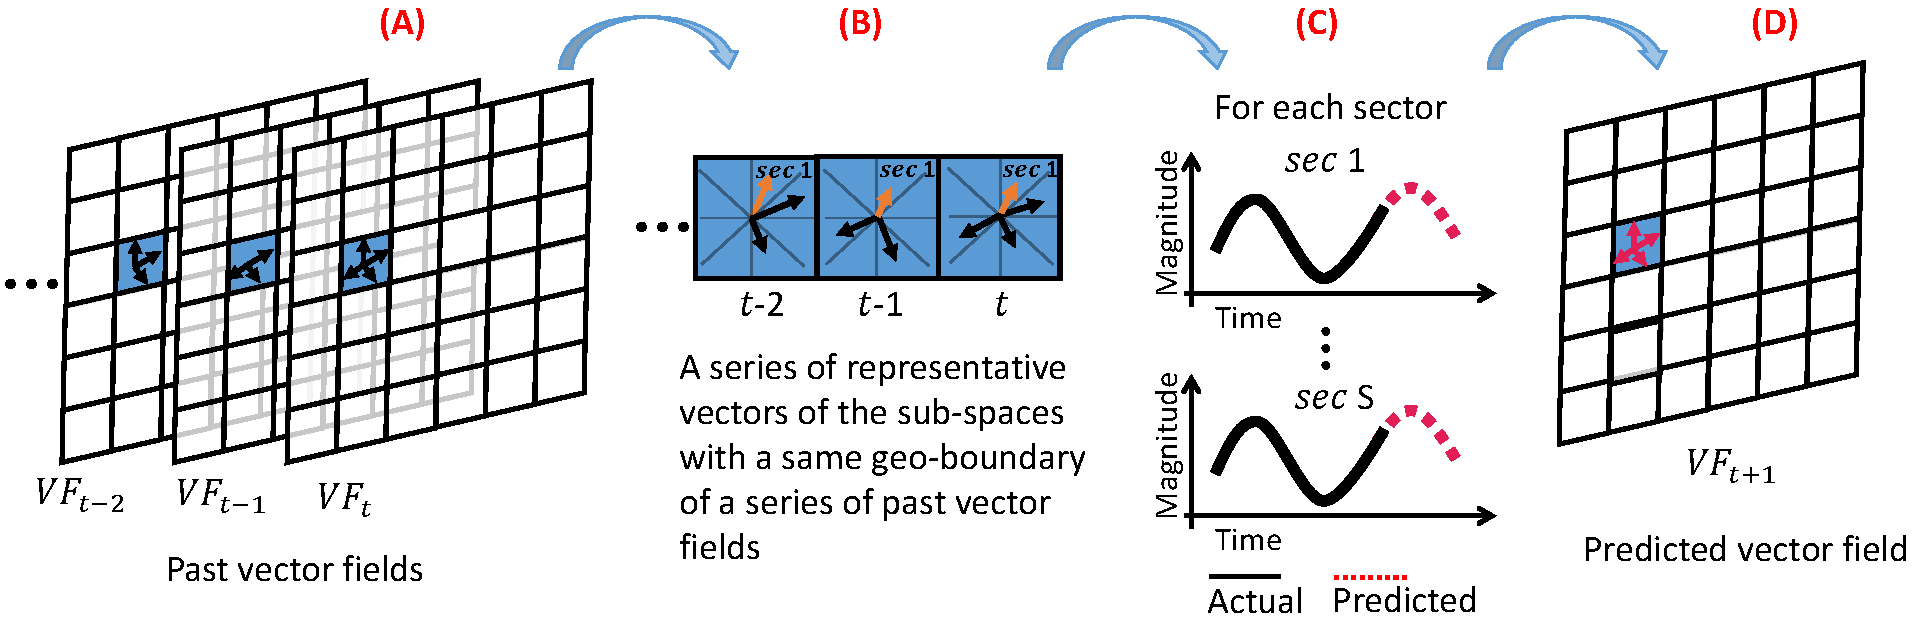
\includegraphics[width=1.0\linewidth]{forecasting_v2}
	\caption{The process of multi-vector field prediction. 
	%We generate a series of the past vector fields (A). a set of smoothed representative vectors for each individual sub-space and A time series vectors are considered to generate a series of representative vectors for each sub-space as shown in (B). (C) for each sector, magnitudes are computed based on STL to have final representative vectors in each space (D).  
	}
	\label{fig:forecasting}
	%\vspace{-0.7cm}
\end{figure*} 

To forecast directional density using historical vector-based crowd data, we apply seasonal trend decomposition based on LOESS technique~\cite{Cleveland:1990:SAS} over the entire space. %on each sub-space. % in order to compute history-based representative vectors for the entire space. 
%We forecast the future flow of a space based on the calculated historical directional density for the sub-spaces of the space utilizing a seasonal trend analysis method~\cite{Cleveland:1990:SAS}.
%Our model forecast the future representative vectors for each sectors of each sub-space separately.
%We then combine the forecasted representative vectors resulted in the future flow as a whole for the entire space.
Figure~\ref{fig:forecasting} illustrates the overall process of our forecasting method.
%In our predictive scheme, each data of the directional distribution is treated as a separate time series variable.
%\textbf{Creating past vector fields:}
For a given geo-location boundary~$\Omega$ and a past time window $t$, 
%(e.g., by day, week) 
we first prepare 
the geospace with the trajectory data (Figure~\ref{fig:forecasting}~(A)).
Next, we fragment the geospace~$\Omega$ into sub-spaces and compute a set of smoothed representative vectors for each individual sub-space using the methodology described in Sections~\ref{sec:discretization} and~\ref{sec:smoothing}.
%As described in Section~\ref{sec:discretization} and ~\ref{sec:smoothing}, then we calculate a set of smoothed representative vectors for each individual sub-space of the space.
%Compared to conventional methods where one vector is assigned to a sub-space for generating a vector field,
%Conventionally, one vector is assigned to a sub-space for generating a vector field.
As discussed previously, we 
%we instead 
calculate a set of representative vectors $\vec{V_k}$ for each sub-space in order to create a multi-vector field (i.e., we calculate representative vectors for each sector of the sub-space (Figure~\ref{fig:forecasting}~(A))).
This is shown in Figure~\ref{fig:forecasting}~(A). % called a multi-vector field.
In our approach, we define these vector fields for the given time window $t$ as 
$VF_t = \left\{\mathcal{M}_{sp_{i}}, \enspace sp_{i} \in \Omega \right\}$, 
where $\mathcal{M}_{sp_{i}}$ is a set of smoothed representative vectors for sub-space $sp_i$.
%for a time window $t$ (e.g., a day), such a vector field is defined as $VF_t = \left\{\mathcal{M}_{sp_{i}}, \enspace sp_{i} \in \Omega \right\}$, where $\mathcal{M}_{sp_{i}}$ is a set of smoothed representative vectors for a sub-space $sp_i$.
%$\Delta{duration}$ is the time duration of the time window (e.g., 3 hours),
This process is repeated for each sub-space in geospace for a given time step, and then over time for the entire time window $t$ (Figure~\ref{fig:forecasting}~(B)). 
%We repeatedly shift the time window $t$ backward and create multi-vector fields for time window $t$ (Figure~\ref{fig:forecasting} (A)) [ISN'T THIS REPETITIVE?].
%\textbf{Extracting series of representative vector sets:}
%Next, we extract a series of $\mathcal{M}_{sp_{i}}$ for each sub-space 
%with a same geo-boundary 
%from the historical multi-vector fields (Figure~\ref{fig:forecasting} (B)).
%\textbf{Preparing time series and forecasting:}
Next, we generate a time series of the \textit{magnitude} values of the representative vectors of the series of $\mathcal{M}_{sp_{i}}$ for each sector of the sub-space (Figure~\ref{fig:forecasting}~(C)).
%that result in $S$ (the number of divided sectors) time series (See Figure~\ref{fig:forecasting} (C)) \textcolor{red}{[???TOO LONG].}
%For a sub-space $sp_i$, 
This time series is defined as:
\begin{equation}
Y_k = \left\{M(\vec{V_k}): \vec{V_k} \in \mathcal{M}_{sp_{i}}, \mathcal{M}_{sp_{i}} \in VF_t, t \in T\right\}, k = \left\{1, \cdots, S\right\}
\end{equation}
Here, $T$ is the time range of observed historical data. % [ARE THE REST OF THE TERMS DEFINED PREVIOUSLY?].

In order to model the time series $Y_k$ and forecast for the future value, we employ the seasonal-trend decomposition technique (STL) described in~\cite{Maciejewski:2011:Forecasting, Malik:2014:Proactive}. 
The technique is based on a locally weighted regression (loess) methodology (STL)~\cite{Cleveland:1990:SAS}.
For each sub-space, we predict the future magnitude value of the representative vector (Figure~\ref{fig:forecasting}~(C)).
%resulted in a set of the predicted representative vectors for the sub-space (See Figure~\ref{fig:forecasting} (D)). \textcolor{red}{[???]}
Finally, we repeat this process for every single sub-space and their corresponding sectors, and generate the future multi-vector field $VF_{t+1}$ (Figure~\ref{fig:forecasting}~(D)).

%Our model repeat to create such vector field a space for a past time interval.
%then prepares a series of such vector fields for a series of the corresponding past time intervals.
%for a certain past period of time frames,

%\begin{enumerate}
	%\item Creating a series of VFs for a certain past period of time frames,
	%\item Extracting a series of vectors from the cells with a same coordinate from the series of VFs,
	%\item Generating two time series, directions and magnitudes, of the series of vectors,
	%\item Applying a temporal prediction method to the two time series for predicting the direction and the magnitude of the future \item vector of the coordinate, and
	%\item Repeating the same procedure on each coordinate to create the future VFs.
%\end{enumerate}


%Forecasting analysis of multiple vector fields using STL

\begin{figure}[tb]
	\centering
	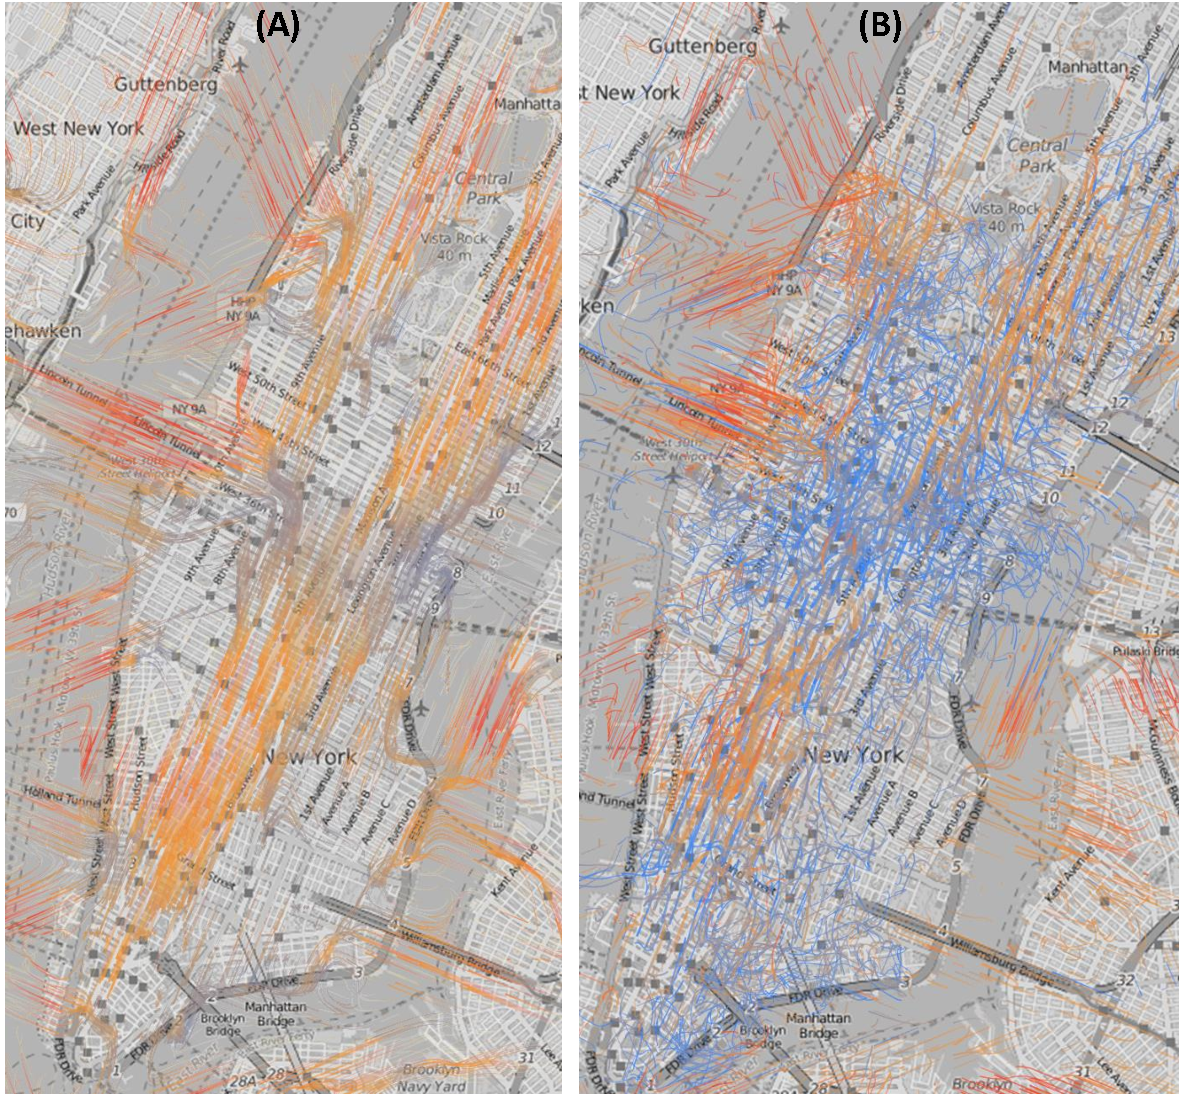
\includegraphics[width=1.0\columnwidth]{twitter_flow}
	\caption{The Major (A) and probability flows (B) of Twitter data between 6:00 AM and 10:00 AM. Note that the probability of a path is accumulated multiplicationaly from the particle birth, the probability in the probability flows might be different from one in the major flows.}
	\label{fig:twitter_flow}
	%\vspace{-0.7cm}
\end{figure}

\begin{figure}[tb]
	\centering
	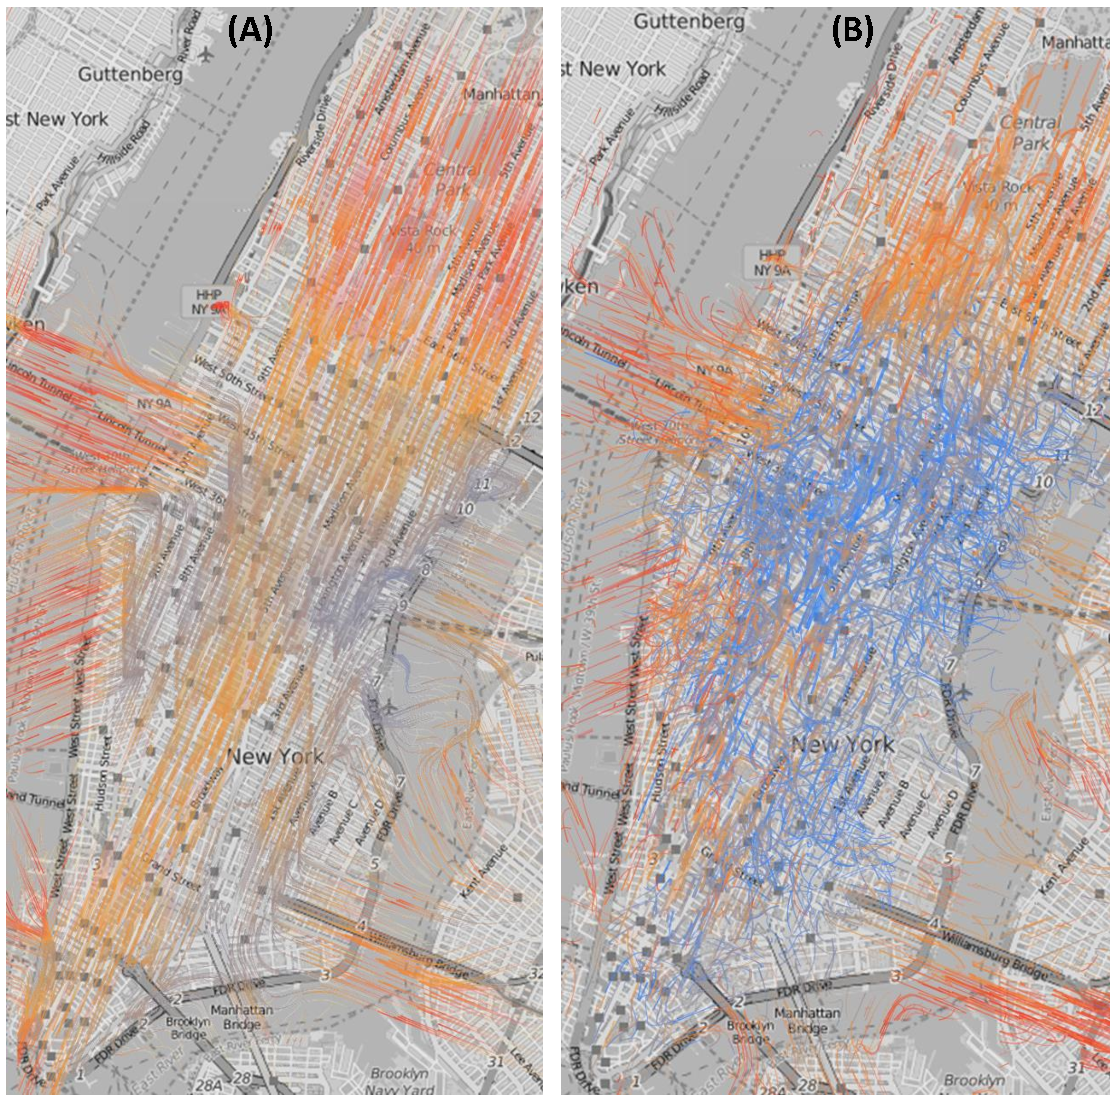
\includegraphics[width=0.93\columnwidth]{twitter_flow_prediction}
	\caption{Forecast Result: The Major (A) and probability flows (B) of Twitter data between 6:00 AM and 10:00 AM. }
	\label{fig:twitter_flow_prediction}
	%\vspace{-0.7cm}
\end{figure}


\subsection{Visualization of Multi-Vector Fields}
\label{sec:forecasting-visualization}

The flow of human crowds represents the temporal trend of human movement within a certain time period. 
Our system is built on several vector field visualization techniques on the generated multi-vector field data in order to observe the trends and patterns. 
%Since we extract the trajectory vector fields, it is possible to apply vector field visualization techniques to observe the trend patterns. 
In this work, we utilize the particle advection technique~\cite{Kruger:FLOW:2005} for the vector fields and extend the web based project, {\textit{earth}}, that visualizes global weather conditions~\cite{earth:2015:online}. 
%
Our web-based flow visualization system consists of JavaScript and several APIs, such as \textit{D3.js}, \textit{Backbone.js}, and \textit{When.js}. The web server visualizes the 3D~globe on the web based according to the vector fields using D3 projections. The server, then, attaches some minimum geographical information including roads, country boundaries, and lakes using the \textit{TopoJSON}. The web-based flow visualization provides animated particles and the color of a particle varies accordingly as the particle ages. If the target vector field area is too small to be visible, our system allows users to apply an additional map of the different map layer located between the globe layer and the particle layer.


\begin{figure*}[tb]
	\centering
	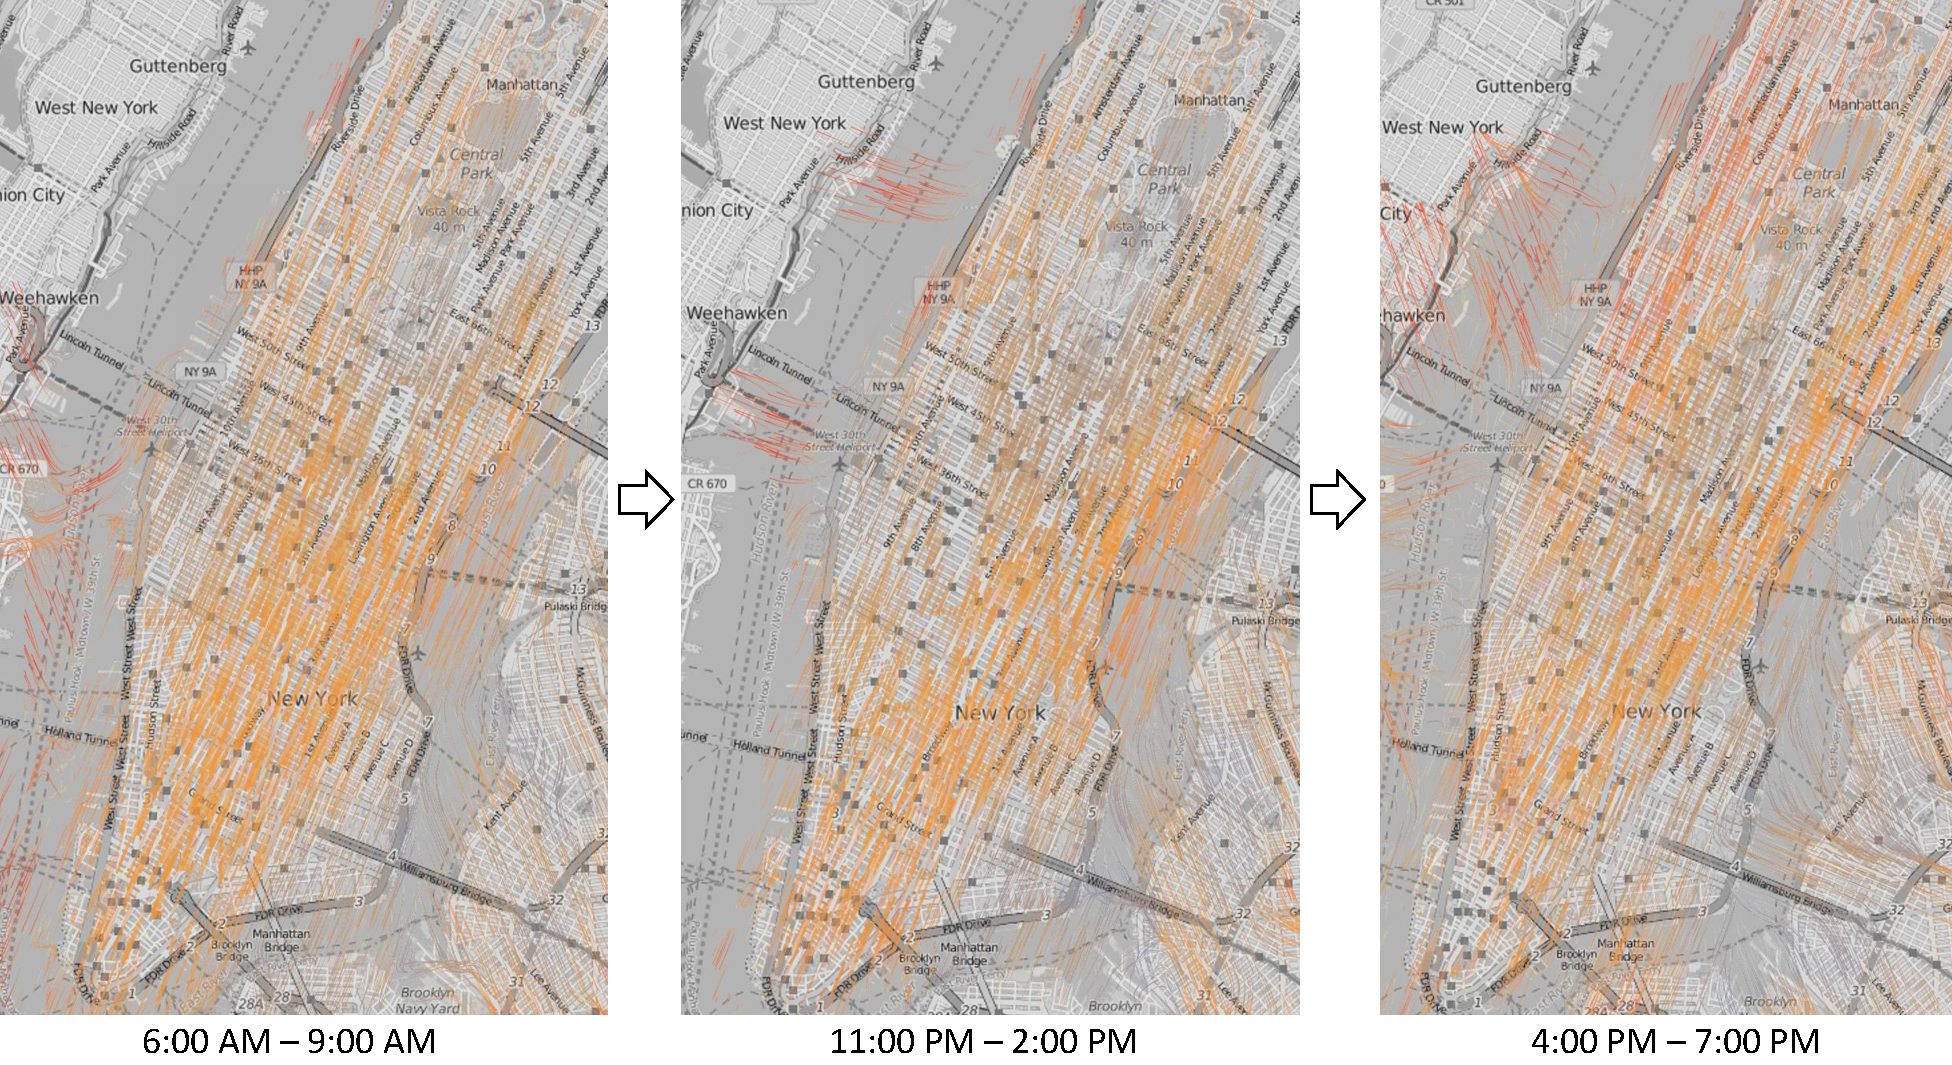
\includegraphics[width=1.0\linewidth]{case_study}
	\caption{The taxi flows of multiple different time frames in a day in Manhattan. It shows the major flow of taxi data during 6:00 AM – 9:00 AM (Left), 11:00 PM – 2:00 PM (Middle), and 4:00 PM – 7:00 PM (Right) on May 30, 2013.}
	\label{fig:case_study_taxi}
	%\vspace{-0.7cm}
\end{figure*} 


In Section~\ref{sec:discretization}, we introduce the directional density estimation to preserve the original vector directions instead of one dominant or average direction. Each direction has a density giving a hint for the probability of moving toward the direction. Since 8 sectors is set in each grid cell for the directions in this work, the densities for the 8 directions can be normalized and used as a probability. Moreover, a direction with high probability indicates that a flow is moving toward the direction with certainty, whereas, a flow moving to a direction with low probability becomes the uncertain flow. 

In order to represent the multi-vector fields in our flow visualization, particles are generated in the space and animated through the vector fields. The particle color is determined by the probability of the movement direction of the particle, where the color varies from the red to the blue gradually. The red indicates a high probability, whereas, the blue represents a low probability. Since the color is probability based, we can say that the red particle paths are more certain and the blue particle paths are relatively uncertain. In addition, since the number of samples utilized to compute the multi-vector field vary over the space, the number of samples are encoded as the intensity of the vector field. We visualize the intensity information in the width of the particle path (i.e., the wider paths indicate a larger group movement). For the vector directions, we animate the particles and fade out the tails to stress the current positions of the particles. 

Our system provides two different visualization modes for the multi-vector fields. One is a major flow and the other is a probability flow. The major flow is obtained by moving the particles toward the highest probability direction within a grid cell and the paths are colored with the highest probability within the cell. An example of the major flow is presented in Figure~\ref{fig:twitter_flow}~(A). Since each grid cell has only one possible direction, the flow fields are relatively smooth. Note that all colors are interpolated along the paths so that there is not abrupt color change. 

On the other hand, the probability flow is created based on the probabilities in the multi-vector field. Particles are randomly generated in the space and they move toward all non-zero directions in the multi-vector field. The number of particles in a given direction is proportional to the probability. For example, if there are two non-zero vectors (90\% and 10\%) in the multi-vector field and 100 particles are passing through the grid cell, 90 particles move in the 90\% vector direction, whereas, 10 particles move in 10\% vector direction. In addition, when a particle enters a new cell, the probability of the particle path is multiplied by the previous probability. In this way, we can compute all probabilities along the particle path from its birth to the death. The probability of each path segment is encoded in the path color as mentioned above. An example of probability flow is shown in Figure~\ref{fig:twitter_flow}~(B). Since the particle path is obtained by using multi-vector fields, the probability flow tends to become complex as all combinations of the flow directions between grid cells are visualized at the same time. Nonetheless, the color represents the certainty/uncertainty of the flow based on the probability of the path segment. Note that the width of the path segment represents the intensity of the vector field, which is proportional to the number of samples toward the direction as mentioned above. 




\section{Case Study}
%\label{sec:case_study}

In this section, we describe the datasets used in this experiment and the experiment environment.
Also, we report the results of our forecasting model.
In our experiments, our model was able to efficiently forecast the flow of human crowds by using three datasets: (1)~Trajectory data extracted from Twitter, (2)~Human trajectory data (GeoLife) ~\cite{Zheng:2009:Mining}, and (3)~Taxi location data~\cite{NYC:2016:Taxi}.
Details on these three datasets have been provided in this section. 
%We now provide details on these ... WHAT?

\subsection{Twitter Data}
%A growing number of people use using 
Location-based social network services (e.g., Twitter, Instagram) have become ubiquitous in the modern age.
They create geo-located data and share this information about their immediate surroundings using smart phones with GPS.
Such spatiotemporal data is also a great data source to understand human mobility.
In this work, we use geo-located twitter data.
We mainly focus on the data generated within Manhattan.
Figure~\ref{fig:twitter_flow} shows an example of the flow results from Twitter data generated in the morning between 6:00 AM - 10:00 AM of August 30th, 2014.
We can see major flows toward from top-right to bottom-left and gathering at the center of Manhattan (See Figure~\ref{fig:twitter_flow} (A)).
Figure~\ref{fig:twitter_flow} (B) shows the probability flow of the same region.
We can see high uncertainty around the center as complex movements.
Figure~\ref{fig:twitter_flow_prediction} shows the forecast result of the same time window as the result of Figure~\ref{fig:twitter_flow}.
The forecast results of the two visualization show significantly similar patterns to the actual result patterns.



\subsection{GeoLife Data: GPS Trajectory Data}

The GeoLife GPS Trajectory Dataset~\cite{Zheng:2009:Mining} contains a total of 18,670 trajectories from 182 users recorded by Microsoft Research Asia (MSRA) in the Beijing from April 2007 to August 2012.
As the data has a high degree of sparseness, we use a longer time window unit (8 hours) and a longer range of historical data (150 days) than with the other example datasets.
Also, when the grid size is less than 500 meters, we cannot compute the future flows, because the size created too many sub-spaces with no data (trajectory).
Figure~\ref{fig:geolife_example} shows an example of the flow results from GeoLife data generated during the evening between 4:00 PM - 10:00 PM on April 22nd, 2009.
The MSRA is located in the center of the highlighted region in Figure~\ref{fig:geolife_example}.
Figure~\ref{fig:geolife_example}~(A) shows the traffic leaving the MSRA campus, because the observed time window is the evening.
The flows of Figure~\ref{fig:geolife_example}~(B) shows the forecast result of the same time window.
We can see also similar pattens in the both actual and forecast flows.
We zoom into the region highlighted in Figure~\ref{fig:geolife_example} and show the probability flow of the zoomed region in Figure~\ref{fig:geolife_msra}.
The flow appears to show masive complex movements around this area.

\begin{figure*}[tb]
	\centering
	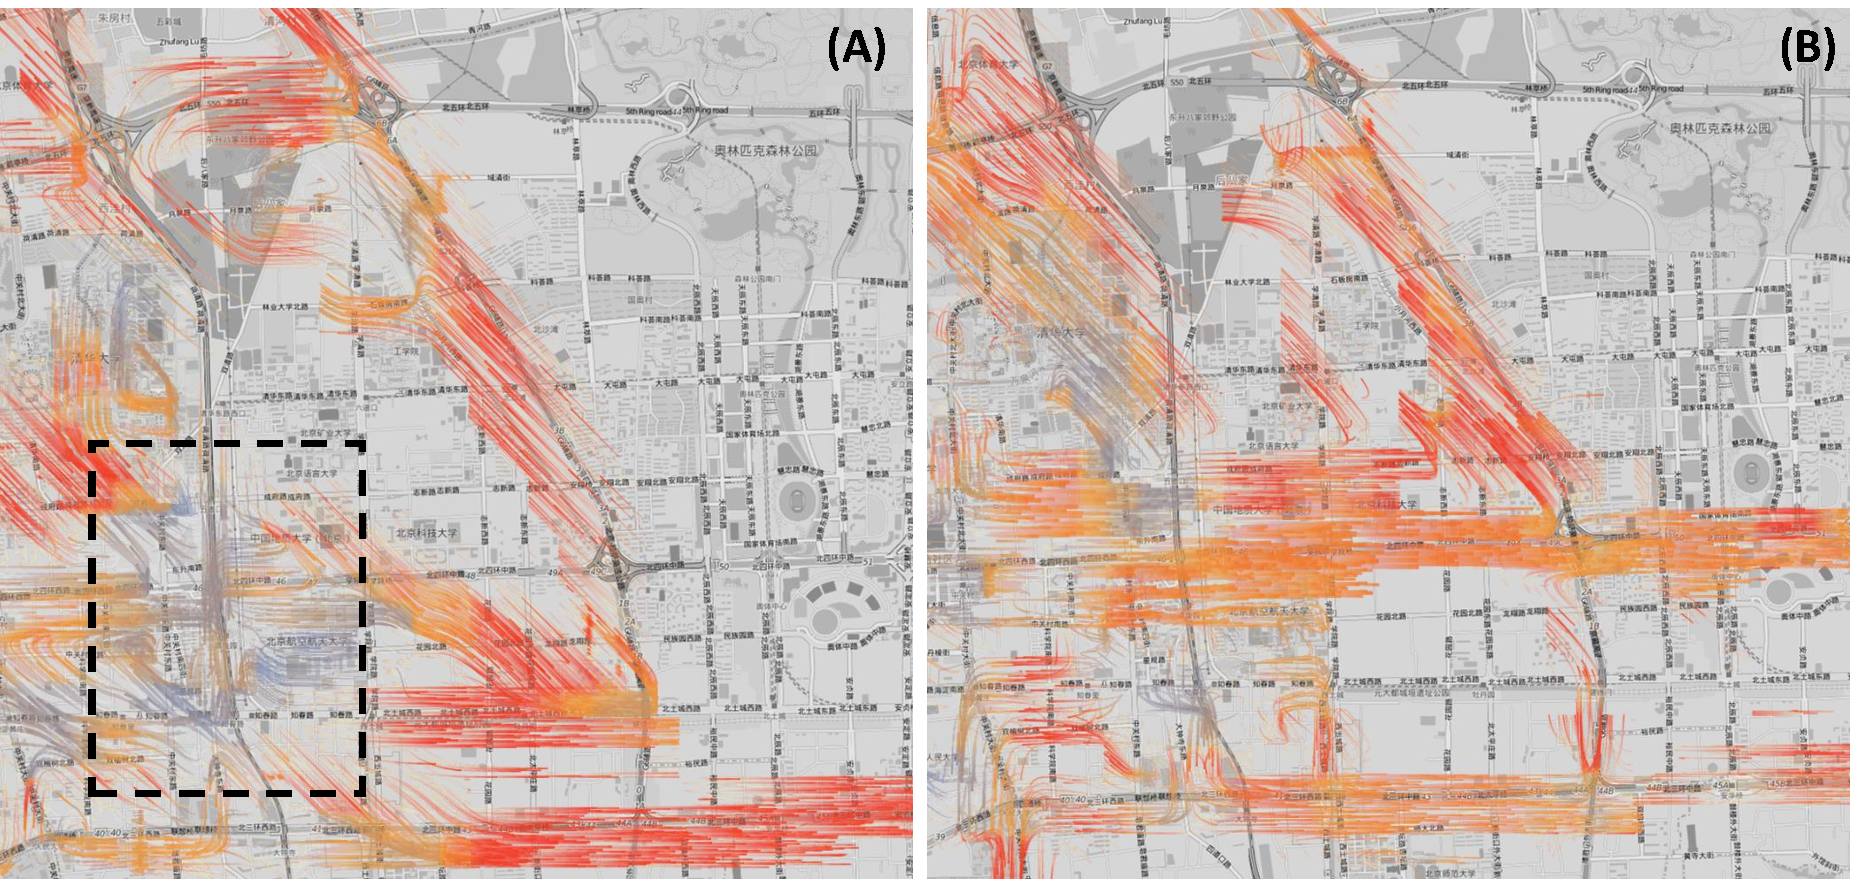
\includegraphics[width=1.0\linewidth]{geolife_example}
	\caption{Flow around the MSRA campus located in the center of the highlighted region. It shows the major flow from GeoLife data during the evening between 4:00 PM - 10:00 PM on April 22nd, 2009. Actual Flow (A) and Forecast Flow (B)}
	\label{fig:geolife_example}
	%\vspace{-0.7cm}
\end{figure*}


\begin{figure}[tb]
	\centering
	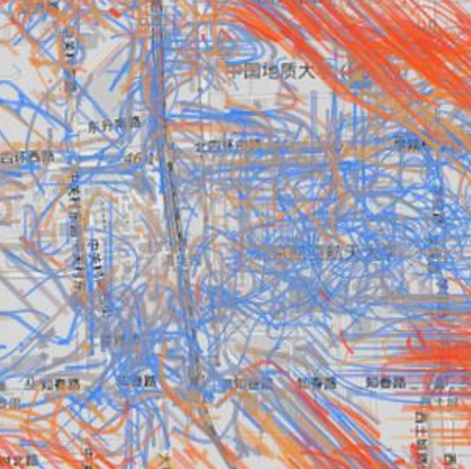
\includegraphics[width=0.6\columnwidth]{geolife_msra}
	\caption{The probability flow zoomed in the MSRA campus}
	\label{fig:geolife_msra}
\end{figure}


\subsection{New York Taxi Data}

The taxi data collected by the New York City (NYC) Taxi and Limousine Commission contains historical taxi trips in NYC, with an average of 500,000~trips per day~\cite{NYC:2016:Taxi}.
Each trip includes passenger pickup and drop-off locations and times, along with other meta data (e.g., trip distance, fare amount).
To demonstrate our work, we utilize the location and time information from the taxi data and focus mainly on trips that took place in Manhattan in 2013.
%For Twitter and taxi data, we looked at the same geo-boundary.
%The taxi data has a more frequent sampling rate than the Twitter data, and the 
%has less uncertainty than twitter data, we used the taxi data for verify results from twitter data.
%We can see the results from both datasets are very similar patterns [FIGURE].
We utilize 1 year of historical data (aggregated by day), and filter the data for portions of the day (i.e., by hour-of-the-day) and utilize our forecasting methodology described in Section~\ref{sec:futureflow}.
We generate these forecasts for three time ranges for 5/30/2013 (Monday): (1) Morning rush hour (6~am~-~9am) (Figure~\ref{fig:case_study_taxi}~(Left)), (2) Afternoon (lunch) commute (11~am~-~2pm) (Figure~\ref{fig:case_study_taxi}~(Middle)), and (3) Evening rush hour (4~pm~-~7pm) (Figure~\ref{fig:case_study_taxi}~(Right)).

The morning commute results (Figure~\ref{fig:case_study_taxi}~(Left)) show an overall pattern of people moving into the middle and southern regions of Manhattan.
This conforms with what is expected and shows that people commute to the commercial regions of the city.
The evening commute results (Figure~\ref{fig:case_study_taxi}~(Right)) show the opposite patterns, and indicate that people may be traveling from work back to home.
The patterns observed during the lunch hours represents more uncertainty of the flows as shown the highlighted region in Figure~\ref{fig:case_study_taxi}~(Middle).
However, we notice more local trends in these results.
%DISCUSS MORE LOCAL TRENDS HERE.
Figure~\ref{fig:case_study_taxi_sub} shows the probability flow of the area highlighted in Figure~\ref{fig:case_study_taxi}~(Left) within the same time frames.
We also note that the forecasts indicate less taxi traffic utilizing the Lincoln tunnel highlighted in Figure~\ref{fig:case_study_taxi_sub}~(Middle) during the morning and evening rush hours. 
However, the Lincoln tunnel is found to have a higher predicted flow during lunch commute hours (Figure~\ref{fig:case_study_taxi_sub}~(Middle)); thereby, indicating that taxi drivers prefer to avoid the tunnel during the morning and evening rush hours.

\begin{figure*}[tb]
	\centering
	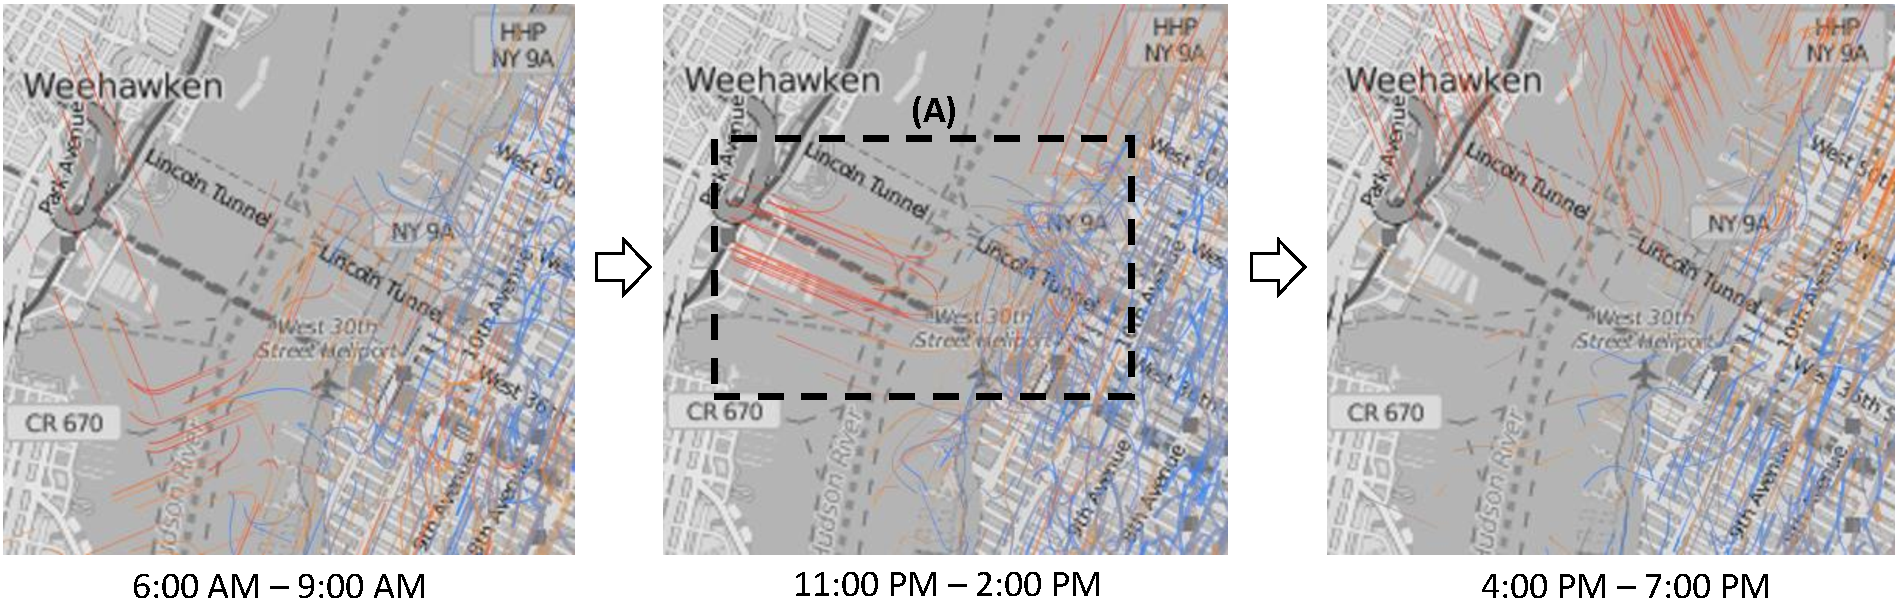
\includegraphics[width=1.0\linewidth]{case_study_sub}
	\caption{The probability flow zoom in around the Lincoln tunnel. Less taxi traffic utilizing the tunnel during the morning (left) and evening (right) rush hours. However, there is a higher predicted flow during lunch commute hours (middle).}
	\label{fig:case_study_taxi_sub}
\end{figure*}


\subsection{Effect of Parameters}

Our trajectory data modeling process for Twitter data introduces several limitations, including issues that arise due to data sparsity. 
In order to mitigate for these challenges, we utilize our flow smoothing approach as described in Section~\ref{sec:smoothing}.
Figure~\ref{fig:LessSmoothing} provide results of applying different global $\tau$ and local $\lambda$ smoothing operations.
The flow with low parameters shows less smooth flow in Figure~\ref{fig:LessSmoothing}~(A) than the flow with high parameter values in in Figure~\ref{fig:LessSmoothing}~(B).

\begin{figure}[tbh]
	\centering
	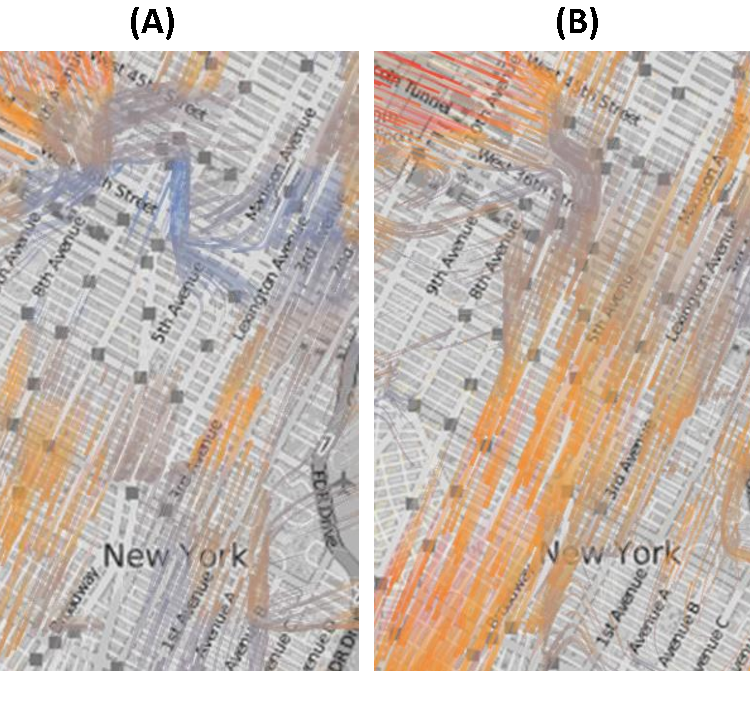
\includegraphics[width=1.0\columnwidth]{LessSmoothing}
	\caption{Smoothing Effect: The flow with the low local smoothing parameter ($\lambda = 0.1$ and $\tau = 0.1$) (A). The flow with the high local smoothing parameter ($\lambda = 0.5$ and $\tau = 0.5$) (B)}
	\label{fig:LessSmoothing}
\end{figure}
\section{Evaluation}

\begin{figure}[tb]
	\centering
	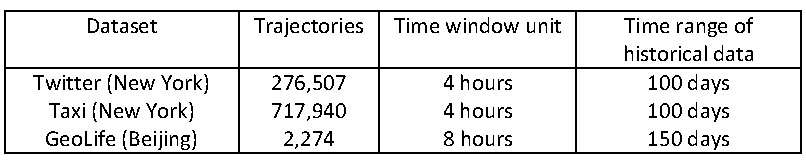
\includegraphics[width=1.0\columnwidth]{Dataset}
	\caption{Experiment environment: We use three different types of datasets. For Twitter and Taxi data, we set the same experiment environment, but for GeoLife data, we set it differently to account for the lower number of daily trajectories.}
	\label{fig:dataset}
	%\vspace{-0.7cm}
\end{figure}

We evaluate the performance of our techniques in terms of the area of each sub-space (e.g., 200m, 500m, 1km, 2km, and 4km) and the number of sectors within each sub-space (4, 6, and 8 sectors) as described in Section~\ref{sec:discretization}. 
%against varying two parameters one a time. 
%Firstly, we vary the grid size (500m, 1km, 2km, and 4km) to investigate the effect of the grid size.
%The second parameter is the number of divided sectors (4, 6, and 8 sectors) to measure the effectiveness of the number of sectors described in Section~\ref{sec:discretization}.
%To evaluate our algorithm, 
%We use two different measures: (1) Normalized Root Mean Square Error (NRMSE)~\cite{Hyndman:2006:Another}, and (2) Mean Absolute Scaled Error (MASE)~\cite{Hyndman:2006:Another}.
%We use the NRMSE measure instead of the Root Mean Square Error (RMSE) to help mitigate for the influence of outliers that generate a low reliability in the evaluation. 
We use Normalized Root Mean Square Error (NRMSE)~\cite{Hyndman:2006:Another} instead of the Root Mean Square Error (RMSE) to help mitigate for the influence of outliers that generate a low reliability in the evaluation and for scale-independent.
The measure is also widely applicable, and easily interpretable. 

%Root Mean Square Error (RMSE) is one of the most popular techniques to measure forecast accuracy~\cite{Hyndman:2006:Another} and NRMSE nomalizes the RMSE. 
%. In this work, we use a family of RMSE, different version, normalizing the RMSE, because RMSE has some drawbacks, such the high influence of outliers in the data and a low reliability.

To compute NRMSE, we first define two time series: (1) Historical time series defined by $Y_k = \left\{y_t: t \in T\right\}$, where $k = \left\{1, \cdots, S\right\}$, and (2) Forecasted time series given by ${\hat{Y}}_k = \left\{{\hat{y}}_t: t \in T\right\}$. 
NRMSE can be calculated as follows:
%In this work, we define NRMSE as
\begin{equation}
NRMSE = \frac{1}{y_{max} - y_{min}}\sqrt {{\frac{{\sum\limits_{{t = 1}}^T {{{\left( {{y_t} - {{\hat{y}}_t}} \right)}^2}} }}{{T}}}}
\end{equation}

%In our experiments, we need to compare the forecast accuracy across time series on different scales. 
%To this end, we also utilize MASE due to its scalability and applicability.  %. The major advantage of MASE is scale-independent. 
%%We first calculate the scaled errors $q_t$ that are defined as:
%The MASE error is calculated using the following equation:
%%The basis for calculating the value of the scaled errors $q_t$ is defined as: 
%\begin{equation}
%MASE = mean(|\frac{{y_t} - {{\hat{y}}_t}}{\frac{1}{T-1} \sum\limits_{{t = 2}}^T | y_t - y_{t-1}|}|)
%\end{equation}
%%The MASE error is then calculated according to:
%%\begin{equation}
%%MASE = mean(|q_t|)
%%\end{equation}
%The error is less than one if the proposed forecast method gives, on average, smaller errors than the one-step error of a naive forecast.
%Conversely, the error is greater than one, the forecasts are worse than the average one-step error.
%DOES THIS MEAN THAT WE ARE AIMING FOR MASE = 1; I.E., THIS IS THE BEST CASE SCENARIO? IF SO, THEN DRAW A THICK LINE ON 1 IN FIGURE.
%We repeat these error measurements 30~times. 
%For each trial, we forecast for different dates and compute the average of all errors.

\textbf{Varying grid sizes:} First, we show the trend in NRMSE with respect to grid sizes (granularity) in Figures~\ref{fig:Chart_NRMSE_Grid}.
For each conditions, we use a fixed number of sectors as~8. 
For GeoLife data, we cannot measure the accuracy when the grid size is less than 500 meters, because of many data sparsity issues in sub-spaces that have no trajectories.
For the Twitter and the Taxi data that have a relatively high trajectory density, we find that both errors increase as the grid size grows.
This shows that a larger area can have high directional uncertainty in forecasting human mobility.
In contrast, for the GeoLife data, the error significantly decreases because the sparsity decreases as the grid size increases.
%For MASE, the size of grid has little effect on the forecast accuracy for the Twitter and Taxi data.
%However, for the GeoLife data, it has a large impact on forecasting accuracy, but the accuracy for the data is still low.
%WHAT DOES THIS TELL ME?? WHAT CONCLUSIONS CAN WE MAKE?
We discuss these results further in Section~\ref{sec:discussion}.

\textbf{Varying sector numbers:} Next, we investigate the effect of the number of sectors on the performance of our technique.
We perform an experiment with three different conditions: 4, 6, and 8 sectors with a fixed grid size of 1~km.
For example, for each sub-space, if we divide one full turn (360\degree) into 4~circular sectors of the same size, each sector will cover 90\degree.
By varying the number of sectors, the NRMSE measure show the forecasting accuracy increase as the number of sectors grows as shown in Figure~\ref{fig:Chart_NRMSE_Sector}.
It proves that our algorithm successfully improve the forecast performance.
%we little impact is observed for forecasting accuracy of the Twitter and Taxi datasets as shown in Figure~\ref{fig:Chart_NRMSE_Sector}.
However, for GeoLife data, the measure shows the error rate increases as the number of sectors grows.
%WHAT DOES THIS SHOW? NEED TO MAKE SOME OBSERVATIONS HERE. 
These results are discussed further in Section~\ref{sec:discussion}.


%\begin{figure}[tbh]
	%\centering
	%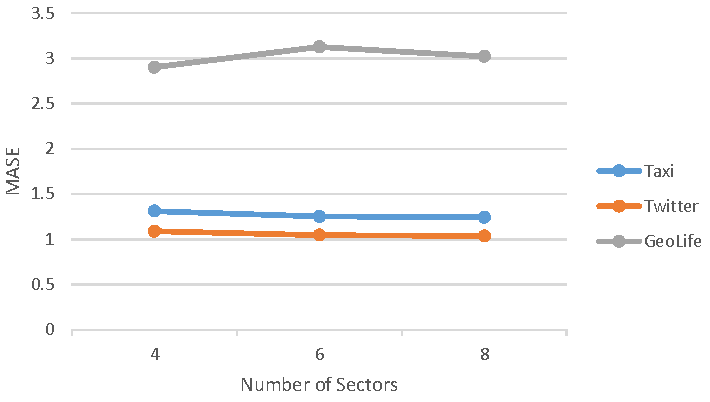
\includegraphics[width=1.0\columnwidth]{Chart_MASE_Sector}
	%\caption{MASE vs the number of sectors}
	%\label{fig:Chart_MASE_Sector}
%\end{figure}


%\begin{figure*}[tbh]
	%\centering
	%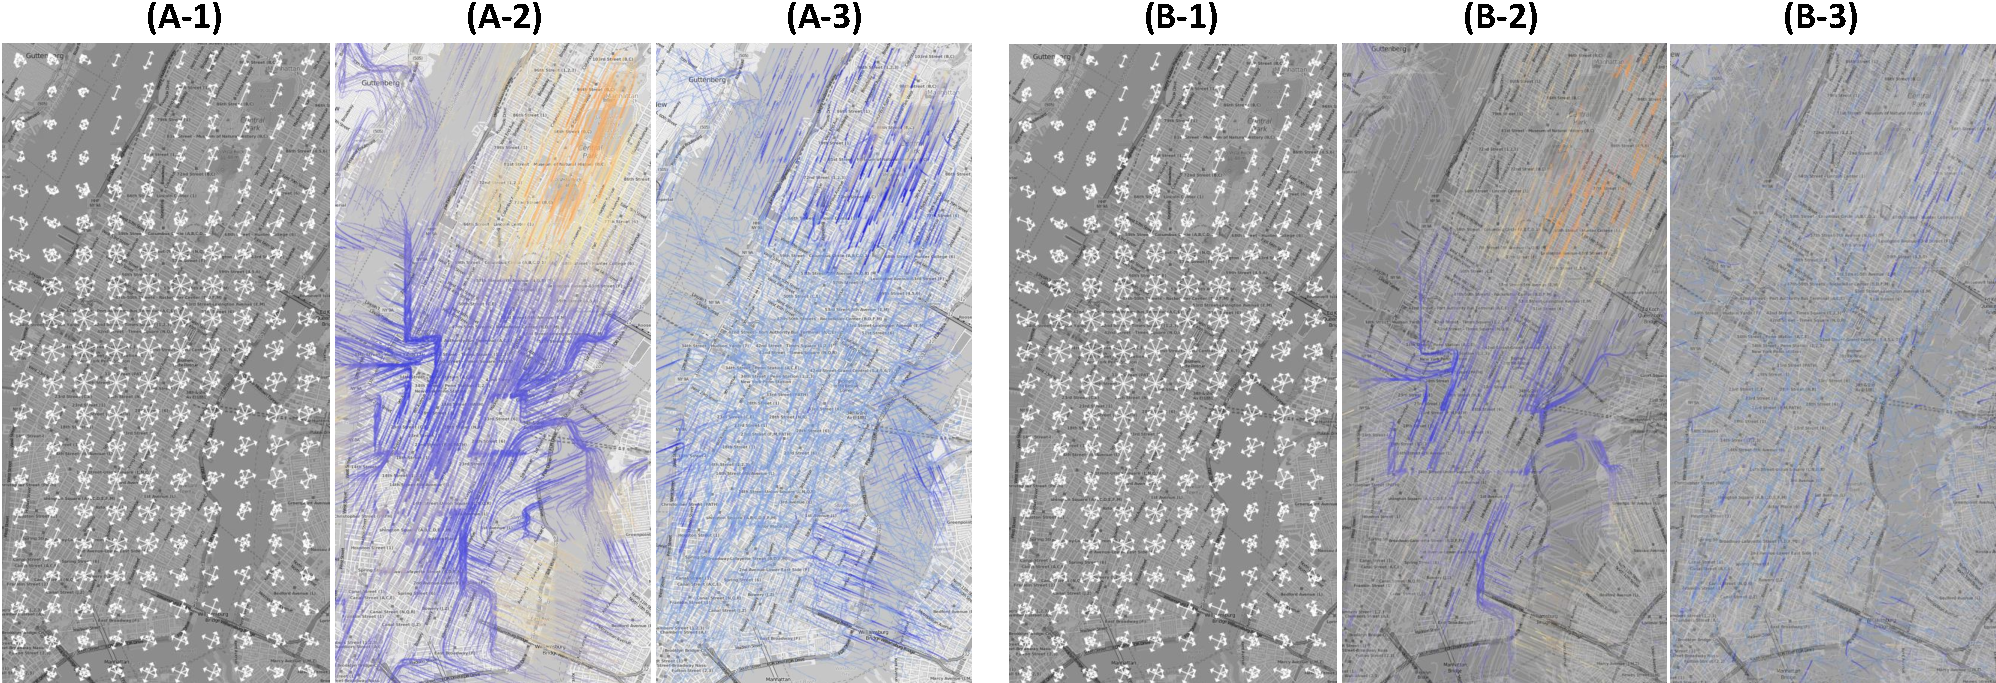
\includegraphics[width=1.0\linewidth]{nyc_forecasting_result}
	%\caption{An example of forecasting result. (A-1) Observed directional density (A-2) Observed major flows (A-3) Observed other flows (B-1) Forecasted directional density (B-2) Forecasted major flows (B-3) Forecasted other flows}
	%\label{fig:forecasting_result}
	%%\vspace{-0.7cm}
%\end{figure*} 
\section{Discussion}
%\label{sec:discussion}

In this section, we discuss issues related to parameter selection for our methodology. % (e.g., grid size, number of sectors, and the visualization).
Specifically, we discuss the challenges associated with selecting the appropriate grid size, number of sectors within sub-space, and the visualization.


\subsection{Grid Size}

As discussed in Section~\ref{sec:discretization}, we conducted our evaluations by varying the grid size.
Our evaluation results reveal that the grid size has an impact on the accuracy of the forecast results.
However, selecting an appropriate grid size (i.e., geospatial scale) for analysis remains to be a challenging task.
%
Based on our experiment results, in general, the data with high density is less vulnerable and the accuracy of forecasting with a higher granularity (coarse scale) is higher than that with low granularity (fine scale). 
One adverse case happens when the grid size is 200 meters where we find that the forecast accuracy is worse than that with 500 meters grid size as shown in Figure~\ref{fig:Chart_NRMSE_Grid}.
Interestingly, this is observed in both Twitter and Taxi data.
%[WHY IS THIS NOT SHOWN IN THE IMAGE??]
%Based on our experiment results, we find that the data with high density provide more accurate results.
%We also find that the forecasting performance using finer scales yield better results than that with coarse scales.
%However, the forecast accuracy with 200 meters is worse than that with 500 meters in both Twitter and Taxi data [WHY IS THIS NOT SHOWN IN THE IMAGE??].
%This situation happens to both Twitter and Taxi data.
Although the two datasets have a relatively higher density than the GeoLife data, the overall geospatial densities of the Twitter data are significantly lower.
%However, the datasets have the same geo-boundary as New York City, a big city.
Accordingly, we believe that there may a relationship between the grid size and the geographical characteristics (e.g., demographics) that needs to be further explored.
We leave this as future work.

%=======
%In this work, we conducted experiments with a number of grid sizes and verified that grid sizes highly impact on the forecast results. In addition, we also confirmed that determining the best grid size is challenging. Based on our experiment results, in general, the data with high density is less vulnerable and the accuracy of forecasting with a higher granularity (less grid size) is higher than that with low granularity. One adverse case happens when the grid size is 200 meters--the forecast accuracy is worse than that with 500 meters grid size. Interestingly, we acquired the same result with both Twitter and Taxi data. Although the two datasets have relatively higher density than that of GeoLife data, their densities are also significantly different. However, the datasets have the same geo-boundary as New York City, one of big cities.
%With these results, we think that there could be relationship between the grid size and geographical characteristics, such as a block size in our algorithms.
%>>>>>>> .r9166

\subsection{Number of Sectors}
In our experiments, we investigated the effect of the number of sectors of the flow forecast accuracy. 
With the high density datasets (Twitter and Taxi data), we find that the number of sectors has impact on the forecasting accuracy as shown in Figure~\ref{fig:Chart_NRMSE_Sector}.
We believe that the smaller number of sectors can cause low directional accuracy
since each divided sector covers a larger range of the direction of vectors when the number of sectors is low. Moreover, we believe that the error rates for the number of sectors are also influenced by the degree of freedom for the movement. If there are many possible paths in a geographical location, the larger number of sectors introduce the less errors. Moreover, the orientations of the representative vectors also affect the error rates according to the number of sectors since a representative vector covers an aggregated direction. We will investigate the optimal number of sectors to minimize the errors as a future work. 
%AM: I FIND THESE FINDINGS STRANGE. LETS DISCUSS THIS IN PERSON TO SEE HOW WE CAN EXPLAIN THIS.  

%But, a higher number of sector requires larger computation for forecasting.


\begin{figure}[t]
	\centering
	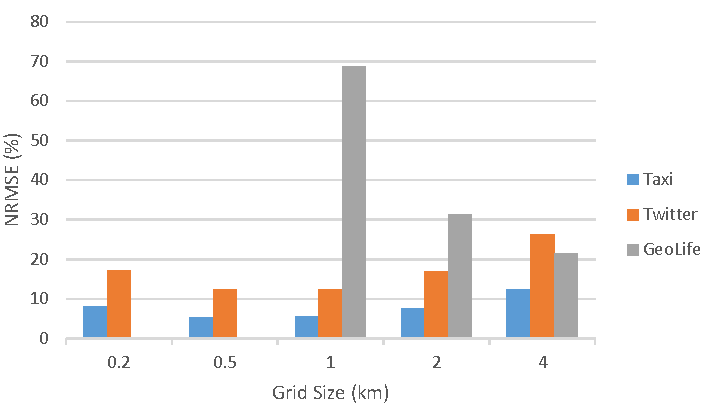
\includegraphics[width=1.0\columnwidth]{Chart_NRMSE_Grid}
	\caption{NRMSE vs the grid size}
	\label{fig:Chart_NRMSE_Grid}
\end{figure}

%\begin{figure}[tbh]
	%\centering
	%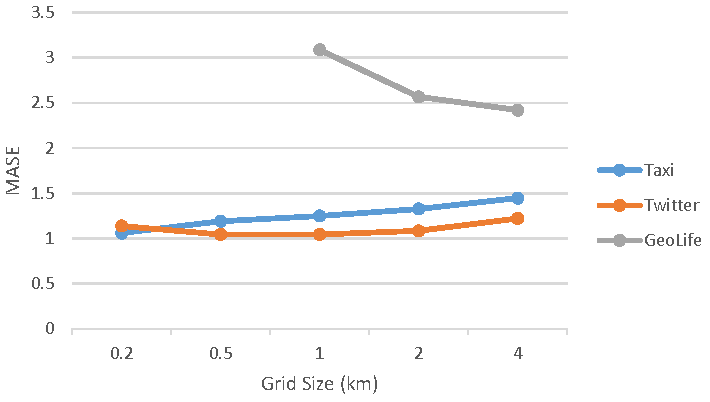
\includegraphics[width=1.0\columnwidth]{Chart_MASE_Grid}
	%\caption{MASE vs the grid size}
	%\label{fig:Chart_MASE_Grid}
%\end{figure}


\subsection{Visualization}
Our flow visualizations are designed to capture the density of each direction. The high density flow is colored in red, while the low density flow is colored in blue. As mentioned in Section~\ref{sec:forecasting-visualization}, the density is treated as the probability of a particle moving toward a direction. As seen in the probability flow in Figure~\ref{fig:twitter_flow}~(B), the low density flow areas tend to have multiple directional uncertain flows, while the high density flow areas have only one or two major certain flows. This indicates that a low density area generates many possible flow paths, but a high density area produces only a few possible flow paths. Therefore, we can differentiate these two flows by the complexity of flow path patterns. Additionally, the major flow provides smoother flows with densities compared to the probability flow. This allows us to observe the overview of the flow vector fields as seen in Figure~\ref{fig:twitter_flow}~(A).

\section{Conclusion and Future Work}

In this paper, we presented a space-based visual analytics approach for forecasting the overall flow of human crowds. 
Our work utilizes individual movement trajectory data and embeds it into a two-dimensional Euclidean space.
Our approach is based on modeling for the space instead of the more conventional approach of modeling individual objects. 
We also propose a new flow smoothing method based on local and global trend estimates in order mitigate for the challenges resulting from data sparseness and noise in the data. 
We utilize the seasonal trend decomposition based on LOESS technique to forecast the future flow using observed historical flow patterns.
We provide several case studies to demonstrate our work. 

Our future work includes factoring in correlations with other datasets in order to further refine our trajectory forecasting methods.
We also plan on incorporating data-driven methods to fragment the geospace based on other features (e.g., road network) instead of only regular grids to compute the forecasts. 
For example, properties of the data may lend themselves well to certain spatial groupings, thereby providing a natural hierarchy for the forecasting. In addition, we will study the influences on the forecasting errors and the optimal forecasting parameters. 
Finally, we plan on further investigating the effects of data sparsity and noise issues on our forecasting results. 


\begin{figure}[t]
	\centering
	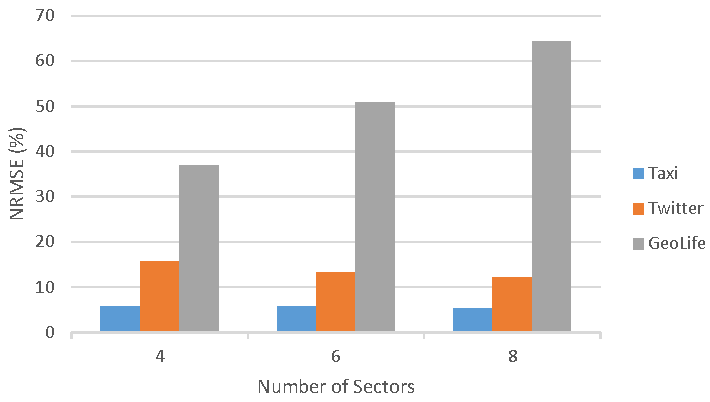
\includegraphics[width=1.0\columnwidth]{Chart_NRMSE_Sector}
	\caption{NRMS vs the number of sectors}
	\label{fig:Chart_NRMSE_Sector}
\end{figure}








